% Main empirical-section paragraph.
Ordinary explained covariance is useful descriptive evidence, but it is not by itself a certificate for a stress functional. Table~\ref{tab:ritz-certification-main} therefore reports both the exact full-coordinate approximation error and the Ritz upper bound for the principal probe in each application at $\lambda_0=1$. The certified rank is probe- and stress-scale-specific: it is the smallest rank for which the maximum deterministic approximation certificate over the reported state set falls below the stated tolerance. All calculations use the same ridge-relative operator, so the rank-$R$ compression uses $(\Lambda_R+\rho I)^{-1/2}$ rather than an unregularized whitening. These bounds are conditional on the estimated covariance operators and do not represent sampling-confidence intervals.

% Application cross-references.
The monetary-policy appendix reports full-coordinate and rank-five stress curves, severe-direction counts, and rank-five capture of high-stress eigenspaces in Figure~\ref{fig:macro-ritz-interval-spectrum}.
The LaLonde appendix validates the Ritz bound directly against the exact 11-coordinate error in Figure~\ref{fig:lalonde-ritz-validation}.
The hurricane subsection reports whether severe amplification is concentrated in one direction or spread over multiple independent directions using Table~\ref{tab:hurricane-ritz-certification}.

% Appendix inclusions.
\begin{table}[!htbp]
\centering
\caption{Finite-rank approximation errors and Ritz bounds}
\label{tab:ritz-certification-main}
\resizebox{\linewidth}{!}{%
\begin{tabular}{@{}llrrrrrr@{}}
\toprule
Application & Probe & $p$ & $R$ & Retained mass & p95 $e_R$ & $\max e_R$ & $\max B_R$ \\
\midrule
LaLonde ATE & overall ATE direction & 11 & 5 & 0.999 & 0.007 & 0.011 & 0.805 \\
Hurricane full fiscal/post probe & fiscal/post block probe & 72 & 5 & 0.661 & 0.178 & 0.214 & 1.000 (vacuous) \\
Hurricane full fiscal/post probe & fiscal/post block probe & 72 & 15 & 0.869 & 0.056 & 0.065 & 1.000 (vacuous) \\
\bottomrule
\end{tabular}
}
\begin{minipage}{0.96\linewidth}
\footnotesize Notes: $e_R$ is the exact full-coordinate stress approximation error at $\lambda_0=1$ and $B_R$ is the capped deterministic Ritz bound. The macro row uses the full-space temporal-resolvent benchmark built from 125-dimensional pre-PCA influence contributions; it is not a full-dimensional latent state-space estimate. Bounds are conditional on the estimated regularized covariance operators.
\end{minipage}
\end{table}


\begin{figure}[!htbp]
\centering
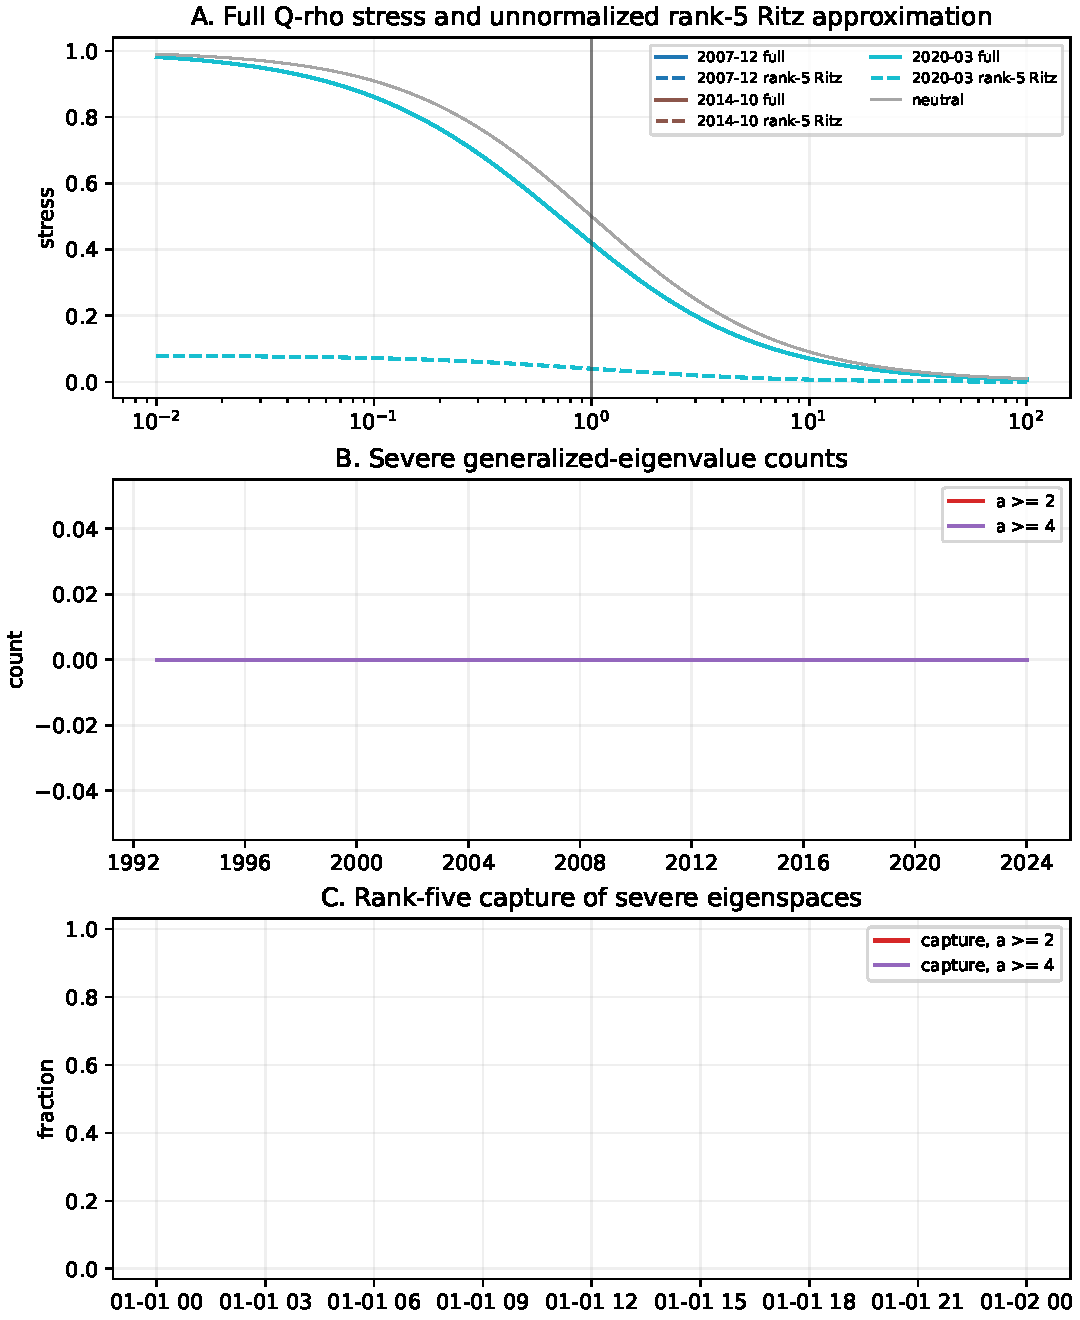
\includegraphics[width=0.96\linewidth]{results/ritz_certification/figures/macro_ritz_interval_spectrum.pdf}
\caption{Macro Ritz stress and interval-spectrum diagnostics. Notes: rank-five stress uses the Ritz matrix from the same ridge-relative operator. Severe-direction counts record generalized eigenvalues above two-times or four-times reference amplification. The ridge parameter, interval backend, and maximum residual are recorded in \texttt{results/ritz_certification/metadata/ritz_certification_metadata.json}.}
\label{fig:macro-ritz-interval-spectrum}
\end{figure}

\begin{table}[!htbp]
\centering
\caption{Hurricane Ritz certification and severe-direction geometry}
\label{tab:hurricane-ritz-certification}
\scriptsize
\textbf{Panel A. Accuracy}\\[0.3em]
\resizebox{\linewidth}{!}{%
\begin{tabular}{@{}llrrrrrr@{}}
\toprule
Surface and rank & Probe & Trace share & Retained mass & p95 $e_R$ & $\max e_R$ & Share $e_R>.05$ & p95 Ritz subspace residual term \\
\midrule
72-coordinate full event-study surface, R=5 & fiscal/post block probe & 0.603 & 0.661 & 0.178 & 0.214 & 0.718 & 2.716 \\
72-coordinate full event-study surface, R=10 & fiscal/post block probe & 0.723 & 0.759 & 0.135 & 0.144 & 0.574 & 4.298 \\
72-coordinate full event-study surface, R=15 & fiscal/post block probe & 0.807 & 0.869 & 0.056 & 0.065 & 0.133 & 3.971 \\
28-coordinate fiscal/post event-study surface, R=5 & whole-surface soft probe & 0.731 & 0.190 & 0.489 & 0.502 & 1.000 & 1.953 \\
28-coordinate fiscal/post event-study surface, R=10 & whole-surface soft probe & 0.902 & 0.379 & 0.366 & 0.373 & 1.000 & 3.490 \\
28-coordinate fiscal/post event-study surface, R=15 & whole-surface soft probe & 0.964 & 0.567 & 0.259 & 0.294 & 0.877 & 2.564 \\
\bottomrule
\end{tabular}
}
\\[0.8em]
\textbf{Panel B. Severe Geometry}\\[0.3em]
\resizebox{\linewidth}{!}{%
\begin{tabular}{@{}lrrrrrr@{}}
\toprule
Surface and threshold & Median $d$ & Max $d$ & Share $d>0$ & Median $\kappa$ & p90 $\kappa$ & Max generalized-eigenpair residual \\
\midrule
72-coordinate full event-study surface, $a_\star=2$ & 10.000 & 23 & 0.959 & 0.013 & 0.144 & 3.2e-13 \\
72-coordinate full event-study surface, $a_\star=4$ & 3.000 & 12 & 0.836 & 0.006 & 0.301 & 3.2e-13 \\
28-coordinate fiscal/post event-study surface, $a_\star=2$ & 2.000 & 15 & 0.621 & 0.108 & 0.337 & 1.4e-13 \\
28-coordinate fiscal/post event-study surface, $a_\star=4$ & 0.000 & 7 & 0.441 & 0.226 & 0.685 & 1.4e-13 \\
\bottomrule
\end{tabular}
}
\begin{minipage}{0.96\linewidth}
\footnotesize Notes: The restricted surface is the true fiscal/post intersection derived from checked-in surface metadata. Panel A's residual term is $r_R(s)/\lambda$ with $\lambda=1$, where $r_R(s)$ is the Ritz subspace residual. Panel B defines $\kappa_5(s;a_\star)=\|V_5'U_\star(s)\|_F^2/d_\star(s;a_\star)$ when $d_\star>0$. Interval eigenpairs are extracted with \texttt{scipy.linalg.eigh(..., subset\_by\_value=...)} and verified against full dense eigenvalue counts; the reported residual is the numerical generalized-eigenpair residual.
\end{minipage}
\end{table}


\begin{figure}[!htbp]
\centering
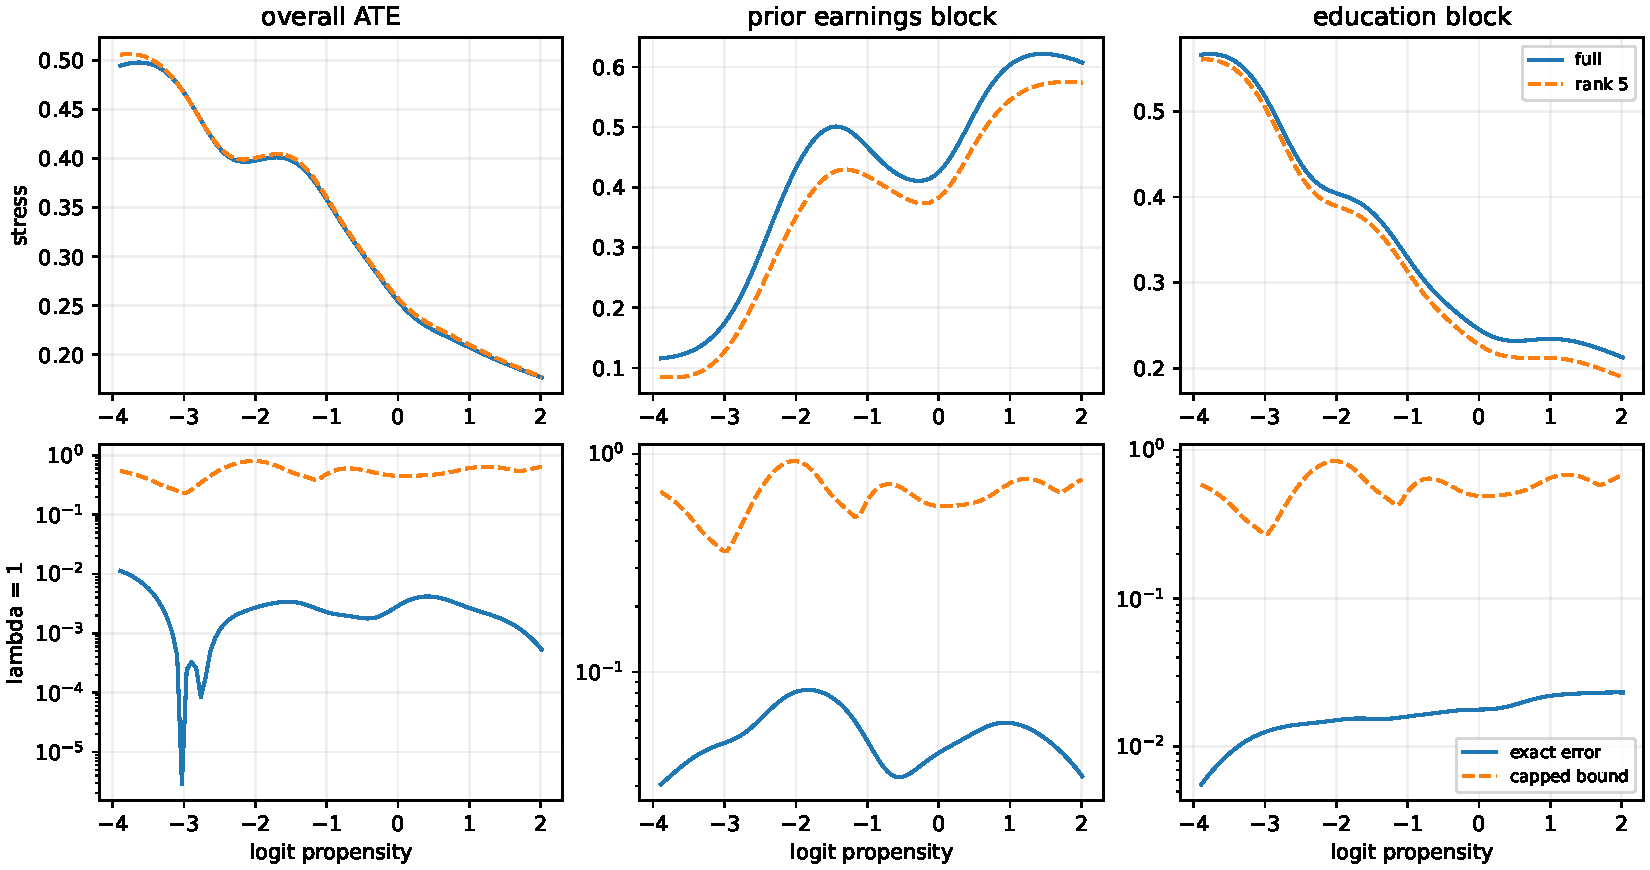
\includegraphics[width=0.96\linewidth]{results/ritz_certification/figures/lalonde_ritz_validation.pdf}
\caption{LaLonde Ritz-bound validation. The low-dimensional LaLonde application permits direct comparison of the exact full-coordinate rank-five error with the deterministic certificate at every plotted propensity-score support point.}
\label{fig:lalonde-ritz-validation}
\end{figure}
